% Created by tikzDevice version 0.9 on 2016-01-12 22:38:52
% !TEX encoding = UTF-8 Unicode
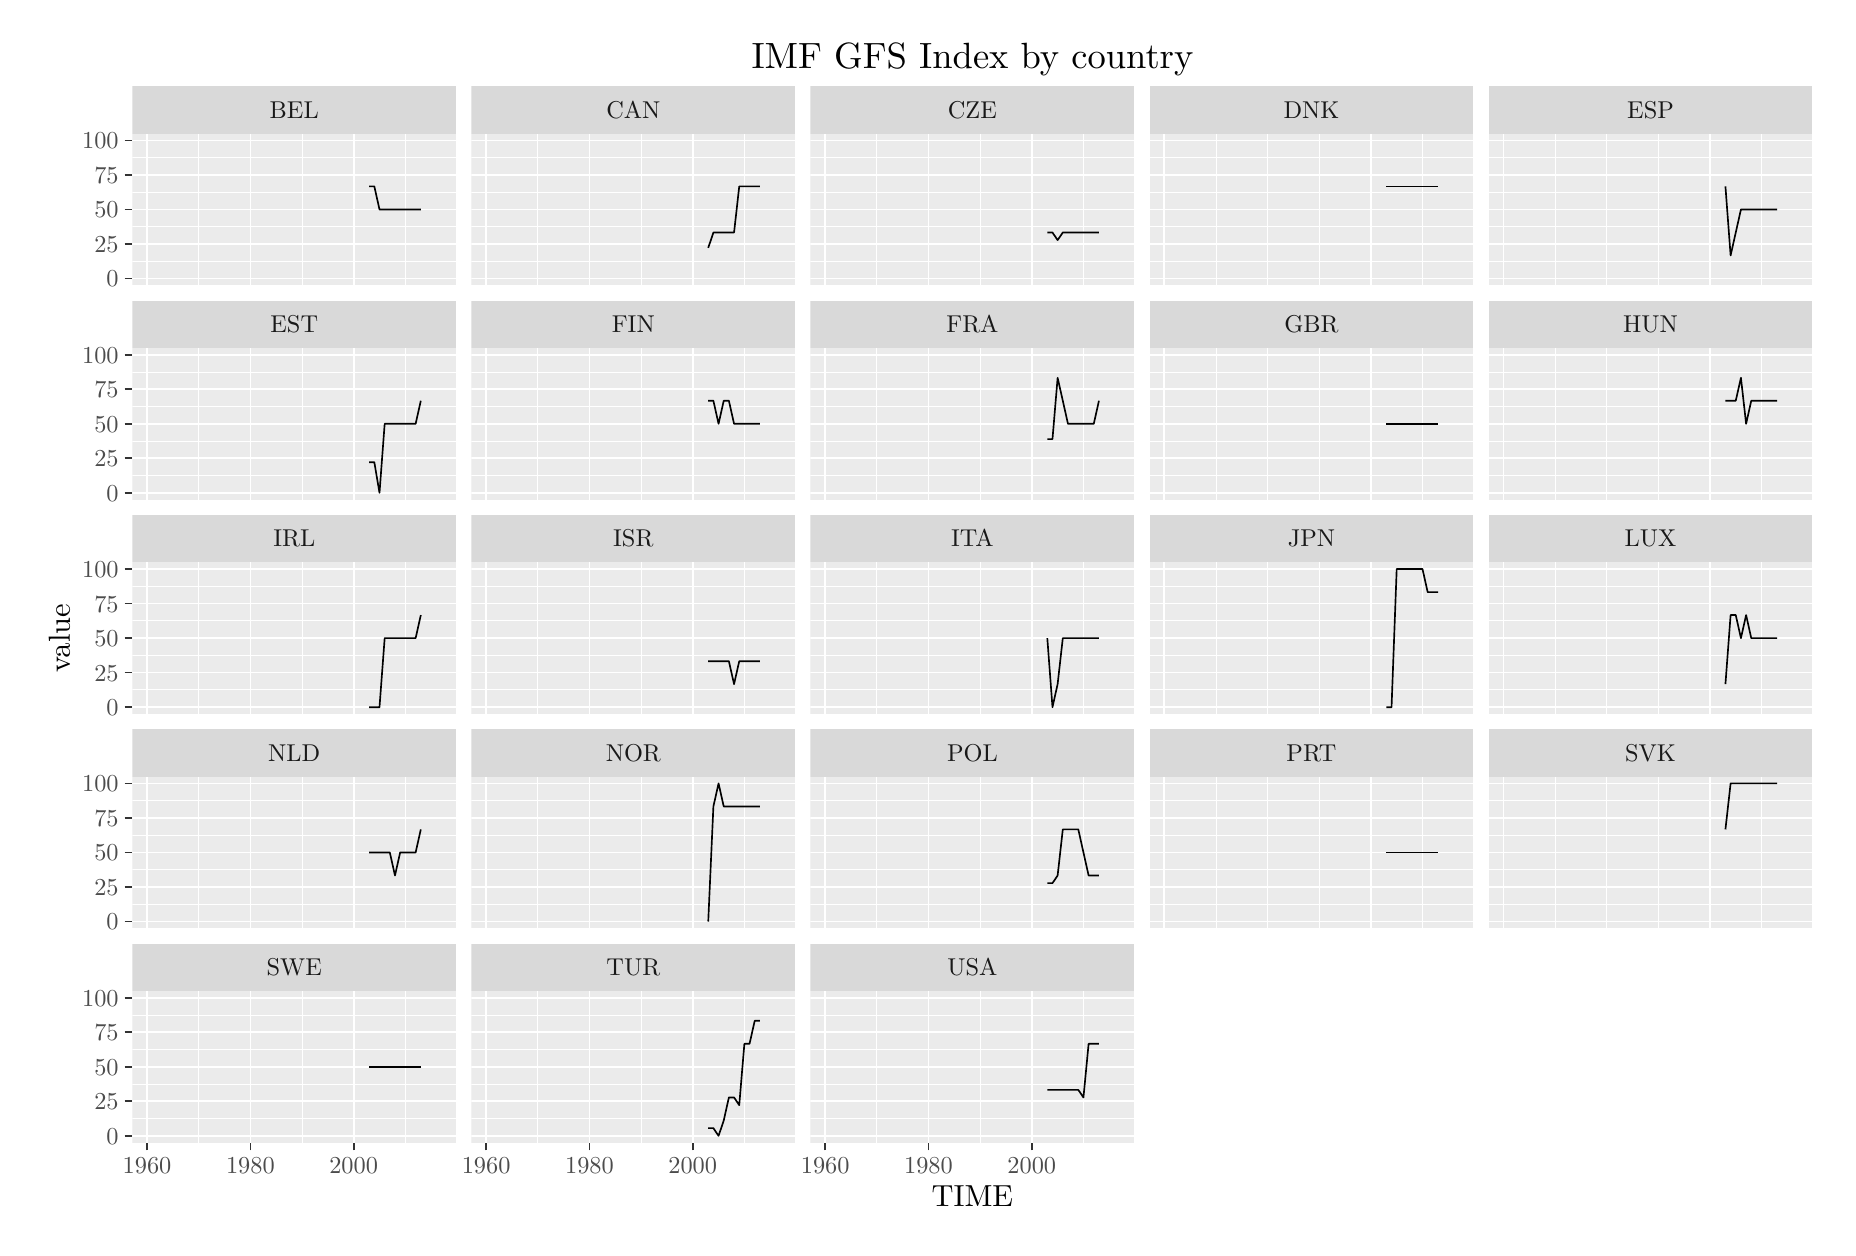
\begin{tikzpicture}[x=1pt,y=1pt]
\definecolor{fillColor}{RGB}{255,255,255}
\path[use as bounding box,fill=fillColor,fill opacity=0.00] (0,0) rectangle (650.43,433.62);
\begin{scope}
\path[clip] (  0.00,  0.00) rectangle (650.43,433.62);
\definecolor{drawColor}{RGB}{255,255,255}
\definecolor{fillColor}{RGB}{255,255,255}

\path[draw=drawColor,line width= 0.6pt,line join=round,line cap=round,fill=fillColor] (  0.00,  0.00) rectangle (650.43,433.62);
\end{scope}
\begin{scope}
\path[clip] ( 37.82,340.48) rectangle (154.84,395.37);
\definecolor{fillColor}{gray}{0.92}

\path[fill=fillColor] ( 37.82,340.48) rectangle (154.84,395.37);
\definecolor{drawColor}{RGB}{255,255,255}

\path[draw=drawColor,line width= 0.3pt,line join=round] ( 37.82,349.21) --
	(154.84,349.21);

\path[draw=drawColor,line width= 0.3pt,line join=round] ( 37.82,361.69) --
	(154.84,361.69);

\path[draw=drawColor,line width= 0.3pt,line join=round] ( 37.82,374.16) --
	(154.84,374.16);

\path[draw=drawColor,line width= 0.3pt,line join=round] ( 37.82,386.64) --
	(154.84,386.64);

\path[draw=drawColor,line width= 0.3pt,line join=round] ( 61.81,340.48) --
	( 61.81,395.37);

\path[draw=drawColor,line width= 0.3pt,line join=round] ( 99.13,340.48) --
	( 99.13,395.37);

\path[draw=drawColor,line width= 0.3pt,line join=round] (136.46,340.48) --
	(136.46,395.37);

\path[draw=drawColor,line width= 0.6pt,line join=round] ( 37.82,342.98) --
	(154.84,342.98);

\path[draw=drawColor,line width= 0.6pt,line join=round] ( 37.82,355.45) --
	(154.84,355.45);

\path[draw=drawColor,line width= 0.6pt,line join=round] ( 37.82,367.92) --
	(154.84,367.92);

\path[draw=drawColor,line width= 0.6pt,line join=round] ( 37.82,380.40) --
	(154.84,380.40);

\path[draw=drawColor,line width= 0.6pt,line join=round] ( 37.82,392.87) --
	(154.84,392.87);

\path[draw=drawColor,line width= 0.6pt,line join=round] ( 43.14,340.48) --
	( 43.14,395.37);

\path[draw=drawColor,line width= 0.6pt,line join=round] ( 80.47,340.48) --
	( 80.47,395.37);

\path[draw=drawColor,line width= 0.6pt,line join=round] (117.80,340.48) --
	(117.80,395.37);
\definecolor{drawColor}{RGB}{0,0,0}

\path[draw=drawColor,line width= 0.6pt,line join=round] (123.40,376.26) --
	(125.26,376.26) --
	(127.13,367.92) --
	(129.00,367.92) --
	(130.86,367.92) --
	(132.73,367.92) --
	(134.59,367.92) --
	(136.46,367.92) --
	(138.33,367.92) --
	(140.19,367.92) --
	(142.06,367.92);
\end{scope}
\begin{scope}
\path[clip] (160.34,340.48) rectangle (277.37,395.37);
\definecolor{fillColor}{gray}{0.92}

\path[fill=fillColor] (160.34,340.48) rectangle (277.37,395.37);
\definecolor{drawColor}{RGB}{255,255,255}

\path[draw=drawColor,line width= 0.3pt,line join=round] (160.34,349.21) --
	(277.37,349.21);

\path[draw=drawColor,line width= 0.3pt,line join=round] (160.34,361.69) --
	(277.37,361.69);

\path[draw=drawColor,line width= 0.3pt,line join=round] (160.34,374.16) --
	(277.37,374.16);

\path[draw=drawColor,line width= 0.3pt,line join=round] (160.34,386.64) --
	(277.37,386.64);

\path[draw=drawColor,line width= 0.3pt,line join=round] (184.33,340.48) --
	(184.33,395.37);

\path[draw=drawColor,line width= 0.3pt,line join=round] (221.65,340.48) --
	(221.65,395.37);

\path[draw=drawColor,line width= 0.3pt,line join=round] (258.98,340.48) --
	(258.98,395.37);

\path[draw=drawColor,line width= 0.6pt,line join=round] (160.34,342.98) --
	(277.37,342.98);

\path[draw=drawColor,line width= 0.6pt,line join=round] (160.34,355.45) --
	(277.37,355.45);

\path[draw=drawColor,line width= 0.6pt,line join=round] (160.34,367.92) --
	(277.37,367.92);

\path[draw=drawColor,line width= 0.6pt,line join=round] (160.34,380.40) --
	(277.37,380.40);

\path[draw=drawColor,line width= 0.6pt,line join=round] (160.34,392.87) --
	(277.37,392.87);

\path[draw=drawColor,line width= 0.6pt,line join=round] (165.66,340.48) --
	(165.66,395.37);

\path[draw=drawColor,line width= 0.6pt,line join=round] (202.99,340.48) --
	(202.99,395.37);

\path[draw=drawColor,line width= 0.6pt,line join=round] (240.32,340.48) --
	(240.32,395.37);
\definecolor{drawColor}{RGB}{0,0,0}

\path[draw=drawColor,line width= 0.6pt,line join=round] (245.92,354.05) --
	(247.78,359.59) --
	(249.65,359.59) --
	(251.52,359.59) --
	(253.38,359.59) --
	(255.25,359.59) --
	(257.12,376.26) --
	(258.98,376.26) --
	(260.85,376.26) --
	(262.71,376.26) --
	(264.58,376.26);
\end{scope}
\begin{scope}
\path[clip] (282.87,340.48) rectangle (399.89,395.37);
\definecolor{fillColor}{gray}{0.92}

\path[fill=fillColor] (282.87,340.48) rectangle (399.89,395.37);
\definecolor{drawColor}{RGB}{255,255,255}

\path[draw=drawColor,line width= 0.3pt,line join=round] (282.87,349.21) --
	(399.89,349.21);

\path[draw=drawColor,line width= 0.3pt,line join=round] (282.87,361.69) --
	(399.89,361.69);

\path[draw=drawColor,line width= 0.3pt,line join=round] (282.87,374.16) --
	(399.89,374.16);

\path[draw=drawColor,line width= 0.3pt,line join=round] (282.87,386.64) --
	(399.89,386.64);

\path[draw=drawColor,line width= 0.3pt,line join=round] (306.85,340.48) --
	(306.85,395.37);

\path[draw=drawColor,line width= 0.3pt,line join=round] (344.18,340.48) --
	(344.18,395.37);

\path[draw=drawColor,line width= 0.3pt,line join=round] (381.50,340.48) --
	(381.50,395.37);

\path[draw=drawColor,line width= 0.6pt,line join=round] (282.87,342.98) --
	(399.89,342.98);

\path[draw=drawColor,line width= 0.6pt,line join=round] (282.87,355.45) --
	(399.89,355.45);

\path[draw=drawColor,line width= 0.6pt,line join=round] (282.87,367.92) --
	(399.89,367.92);

\path[draw=drawColor,line width= 0.6pt,line join=round] (282.87,380.40) --
	(399.89,380.40);

\path[draw=drawColor,line width= 0.6pt,line join=round] (282.87,392.87) --
	(399.89,392.87);

\path[draw=drawColor,line width= 0.6pt,line join=round] (288.18,340.48) --
	(288.18,395.37);

\path[draw=drawColor,line width= 0.6pt,line join=round] (325.51,340.48) --
	(325.51,395.37);

\path[draw=drawColor,line width= 0.6pt,line join=round] (362.84,340.48) --
	(362.84,395.37);
\definecolor{drawColor}{RGB}{0,0,0}

\path[draw=drawColor,line width= 0.6pt,line join=round] (368.44,359.59) --
	(370.31,359.59) --
	(372.17,356.85) --
	(374.04,359.59) --
	(375.90,359.59) --
	(377.77,359.59) --
	(379.64,359.59) --
	(381.50,359.59) --
	(383.37,359.59) --
	(385.24,359.59) --
	(387.10,359.59);
\end{scope}
\begin{scope}
\path[clip] (405.39,340.48) rectangle (522.41,395.37);
\definecolor{fillColor}{gray}{0.92}

\path[fill=fillColor] (405.39,340.48) rectangle (522.41,395.37);
\definecolor{drawColor}{RGB}{255,255,255}

\path[draw=drawColor,line width= 0.3pt,line join=round] (405.39,349.21) --
	(522.41,349.21);

\path[draw=drawColor,line width= 0.3pt,line join=round] (405.39,361.69) --
	(522.41,361.69);

\path[draw=drawColor,line width= 0.3pt,line join=round] (405.39,374.16) --
	(522.41,374.16);

\path[draw=drawColor,line width= 0.3pt,line join=round] (405.39,386.64) --
	(522.41,386.64);

\path[draw=drawColor,line width= 0.3pt,line join=round] (429.37,340.48) --
	(429.37,395.37);

\path[draw=drawColor,line width= 0.3pt,line join=round] (466.70,340.48) --
	(466.70,395.37);

\path[draw=drawColor,line width= 0.3pt,line join=round] (504.02,340.48) --
	(504.02,395.37);

\path[draw=drawColor,line width= 0.6pt,line join=round] (405.39,342.98) --
	(522.41,342.98);

\path[draw=drawColor,line width= 0.6pt,line join=round] (405.39,355.45) --
	(522.41,355.45);

\path[draw=drawColor,line width= 0.6pt,line join=round] (405.39,367.92) --
	(522.41,367.92);

\path[draw=drawColor,line width= 0.6pt,line join=round] (405.39,380.40) --
	(522.41,380.40);

\path[draw=drawColor,line width= 0.6pt,line join=round] (405.39,392.87) --
	(522.41,392.87);

\path[draw=drawColor,line width= 0.6pt,line join=round] (410.71,340.48) --
	(410.71,395.37);

\path[draw=drawColor,line width= 0.6pt,line join=round] (448.03,340.48) --
	(448.03,395.37);

\path[draw=drawColor,line width= 0.6pt,line join=round] (485.36,340.48) --
	(485.36,395.37);
\definecolor{drawColor}{RGB}{0,0,0}

\path[draw=drawColor,line width= 0.6pt,line join=round] (490.96,376.26) --
	(492.83,376.26) --
	(494.69,376.26) --
	(496.56,376.26) --
	(498.43,376.26) --
	(500.29,376.26) --
	(502.16,376.26) --
	(504.02,376.26) --
	(505.89,376.26) --
	(507.76,376.26) --
	(509.62,376.26);
\end{scope}
\begin{scope}
\path[clip] (527.91,340.48) rectangle (644.93,395.37);
\definecolor{fillColor}{gray}{0.92}

\path[fill=fillColor] (527.91,340.48) rectangle (644.93,395.37);
\definecolor{drawColor}{RGB}{255,255,255}

\path[draw=drawColor,line width= 0.3pt,line join=round] (527.91,349.21) --
	(644.93,349.21);

\path[draw=drawColor,line width= 0.3pt,line join=round] (527.91,361.69) --
	(644.93,361.69);

\path[draw=drawColor,line width= 0.3pt,line join=round] (527.91,374.16) --
	(644.93,374.16);

\path[draw=drawColor,line width= 0.3pt,line join=round] (527.91,386.64) --
	(644.93,386.64);

\path[draw=drawColor,line width= 0.3pt,line join=round] (551.89,340.48) --
	(551.89,395.37);

\path[draw=drawColor,line width= 0.3pt,line join=round] (589.22,340.48) --
	(589.22,395.37);

\path[draw=drawColor,line width= 0.3pt,line join=round] (626.55,340.48) --
	(626.55,395.37);

\path[draw=drawColor,line width= 0.6pt,line join=round] (527.91,342.98) --
	(644.93,342.98);

\path[draw=drawColor,line width= 0.6pt,line join=round] (527.91,355.45) --
	(644.93,355.45);

\path[draw=drawColor,line width= 0.6pt,line join=round] (527.91,367.92) --
	(644.93,367.92);

\path[draw=drawColor,line width= 0.6pt,line join=round] (527.91,380.40) --
	(644.93,380.40);

\path[draw=drawColor,line width= 0.6pt,line join=round] (527.91,392.87) --
	(644.93,392.87);

\path[draw=drawColor,line width= 0.6pt,line join=round] (533.23,340.48) --
	(533.23,395.37);

\path[draw=drawColor,line width= 0.6pt,line join=round] (570.56,340.48) --
	(570.56,395.37);

\path[draw=drawColor,line width= 0.6pt,line join=round] (607.88,340.48) --
	(607.88,395.37);
\definecolor{drawColor}{RGB}{0,0,0}

\path[draw=drawColor,line width= 0.6pt,line join=round] (613.48,376.26) --
	(615.35,351.31) --
	(617.21,359.59) --
	(619.08,367.92) --
	(620.95,367.92) --
	(622.81,367.92) --
	(624.68,367.92) --
	(626.55,367.92) --
	(628.41,367.92) --
	(630.28,367.92) --
	(632.15,367.92);
\end{scope}
\begin{scope}
\path[clip] ( 37.82,263.03) rectangle (154.84,317.92);
\definecolor{fillColor}{gray}{0.92}

\path[fill=fillColor] ( 37.82,263.03) rectangle (154.84,317.92);
\definecolor{drawColor}{RGB}{255,255,255}

\path[draw=drawColor,line width= 0.3pt,line join=round] ( 37.82,271.76) --
	(154.84,271.76);

\path[draw=drawColor,line width= 0.3pt,line join=round] ( 37.82,284.24) --
	(154.84,284.24);

\path[draw=drawColor,line width= 0.3pt,line join=round] ( 37.82,296.71) --
	(154.84,296.71);

\path[draw=drawColor,line width= 0.3pt,line join=round] ( 37.82,309.19) --
	(154.84,309.19);

\path[draw=drawColor,line width= 0.3pt,line join=round] ( 61.81,263.03) --
	( 61.81,317.92);

\path[draw=drawColor,line width= 0.3pt,line join=round] ( 99.13,263.03) --
	( 99.13,317.92);

\path[draw=drawColor,line width= 0.3pt,line join=round] (136.46,263.03) --
	(136.46,317.92);

\path[draw=drawColor,line width= 0.6pt,line join=round] ( 37.82,265.53) --
	(154.84,265.53);

\path[draw=drawColor,line width= 0.6pt,line join=round] ( 37.82,278.00) --
	(154.84,278.00);

\path[draw=drawColor,line width= 0.6pt,line join=round] ( 37.82,290.48) --
	(154.84,290.48);

\path[draw=drawColor,line width= 0.6pt,line join=round] ( 37.82,302.95) --
	(154.84,302.95);

\path[draw=drawColor,line width= 0.6pt,line join=round] ( 37.82,315.42) --
	(154.84,315.42);

\path[draw=drawColor,line width= 0.6pt,line join=round] ( 43.14,263.03) --
	( 43.14,317.92);

\path[draw=drawColor,line width= 0.6pt,line join=round] ( 80.47,263.03) --
	( 80.47,317.92);

\path[draw=drawColor,line width= 0.6pt,line join=round] (117.80,263.03) --
	(117.80,317.92);
\definecolor{drawColor}{RGB}{0,0,0}

\path[draw=drawColor,line width= 0.6pt,line join=round] (123.40,276.60) --
	(125.26,276.60) --
	(127.13,265.53) --
	(129.00,290.48) --
	(130.86,290.48) --
	(132.73,290.48) --
	(134.59,290.48) --
	(136.46,290.48) --
	(138.33,290.48) --
	(140.19,290.48) --
	(142.06,298.81);
\end{scope}
\begin{scope}
\path[clip] (160.34,263.03) rectangle (277.37,317.92);
\definecolor{fillColor}{gray}{0.92}

\path[fill=fillColor] (160.34,263.03) rectangle (277.37,317.92);
\definecolor{drawColor}{RGB}{255,255,255}

\path[draw=drawColor,line width= 0.3pt,line join=round] (160.34,271.76) --
	(277.37,271.76);

\path[draw=drawColor,line width= 0.3pt,line join=round] (160.34,284.24) --
	(277.37,284.24);

\path[draw=drawColor,line width= 0.3pt,line join=round] (160.34,296.71) --
	(277.37,296.71);

\path[draw=drawColor,line width= 0.3pt,line join=round] (160.34,309.19) --
	(277.37,309.19);

\path[draw=drawColor,line width= 0.3pt,line join=round] (184.33,263.03) --
	(184.33,317.92);

\path[draw=drawColor,line width= 0.3pt,line join=round] (221.65,263.03) --
	(221.65,317.92);

\path[draw=drawColor,line width= 0.3pt,line join=round] (258.98,263.03) --
	(258.98,317.92);

\path[draw=drawColor,line width= 0.6pt,line join=round] (160.34,265.53) --
	(277.37,265.53);

\path[draw=drawColor,line width= 0.6pt,line join=round] (160.34,278.00) --
	(277.37,278.00);

\path[draw=drawColor,line width= 0.6pt,line join=round] (160.34,290.48) --
	(277.37,290.48);

\path[draw=drawColor,line width= 0.6pt,line join=round] (160.34,302.95) --
	(277.37,302.95);

\path[draw=drawColor,line width= 0.6pt,line join=round] (160.34,315.42) --
	(277.37,315.42);

\path[draw=drawColor,line width= 0.6pt,line join=round] (165.66,263.03) --
	(165.66,317.92);

\path[draw=drawColor,line width= 0.6pt,line join=round] (202.99,263.03) --
	(202.99,317.92);

\path[draw=drawColor,line width= 0.6pt,line join=round] (240.32,263.03) --
	(240.32,317.92);
\definecolor{drawColor}{RGB}{0,0,0}

\path[draw=drawColor,line width= 0.6pt,line join=round] (245.92,298.81) --
	(247.78,298.81) --
	(249.65,290.48) --
	(251.52,298.81) --
	(253.38,298.81) --
	(255.25,290.48) --
	(257.12,290.48) --
	(258.98,290.48) --
	(260.85,290.48) --
	(262.71,290.48) --
	(264.58,290.48);
\end{scope}
\begin{scope}
\path[clip] (282.87,263.03) rectangle (399.89,317.92);
\definecolor{fillColor}{gray}{0.92}

\path[fill=fillColor] (282.87,263.03) rectangle (399.89,317.92);
\definecolor{drawColor}{RGB}{255,255,255}

\path[draw=drawColor,line width= 0.3pt,line join=round] (282.87,271.76) --
	(399.89,271.76);

\path[draw=drawColor,line width= 0.3pt,line join=round] (282.87,284.24) --
	(399.89,284.24);

\path[draw=drawColor,line width= 0.3pt,line join=round] (282.87,296.71) --
	(399.89,296.71);

\path[draw=drawColor,line width= 0.3pt,line join=round] (282.87,309.19) --
	(399.89,309.19);

\path[draw=drawColor,line width= 0.3pt,line join=round] (306.85,263.03) --
	(306.85,317.92);

\path[draw=drawColor,line width= 0.3pt,line join=round] (344.18,263.03) --
	(344.18,317.92);

\path[draw=drawColor,line width= 0.3pt,line join=round] (381.50,263.03) --
	(381.50,317.92);

\path[draw=drawColor,line width= 0.6pt,line join=round] (282.87,265.53) --
	(399.89,265.53);

\path[draw=drawColor,line width= 0.6pt,line join=round] (282.87,278.00) --
	(399.89,278.00);

\path[draw=drawColor,line width= 0.6pt,line join=round] (282.87,290.48) --
	(399.89,290.48);

\path[draw=drawColor,line width= 0.6pt,line join=round] (282.87,302.95) --
	(399.89,302.95);

\path[draw=drawColor,line width= 0.6pt,line join=round] (282.87,315.42) --
	(399.89,315.42);

\path[draw=drawColor,line width= 0.6pt,line join=round] (288.18,263.03) --
	(288.18,317.92);

\path[draw=drawColor,line width= 0.6pt,line join=round] (325.51,263.03) --
	(325.51,317.92);

\path[draw=drawColor,line width= 0.6pt,line join=round] (362.84,263.03) --
	(362.84,317.92);
\definecolor{drawColor}{RGB}{0,0,0}

\path[draw=drawColor,line width= 0.6pt,line join=round] (368.44,284.94) --
	(370.31,284.94) --
	(372.17,307.09) --
	(374.04,298.81) --
	(375.90,290.48) --
	(377.77,290.48) --
	(379.64,290.48) --
	(381.50,290.48) --
	(383.37,290.48) --
	(385.24,290.48) --
	(387.10,298.81);
\end{scope}
\begin{scope}
\path[clip] (405.39,263.03) rectangle (522.41,317.92);
\definecolor{fillColor}{gray}{0.92}

\path[fill=fillColor] (405.39,263.03) rectangle (522.41,317.92);
\definecolor{drawColor}{RGB}{255,255,255}

\path[draw=drawColor,line width= 0.3pt,line join=round] (405.39,271.76) --
	(522.41,271.76);

\path[draw=drawColor,line width= 0.3pt,line join=round] (405.39,284.24) --
	(522.41,284.24);

\path[draw=drawColor,line width= 0.3pt,line join=round] (405.39,296.71) --
	(522.41,296.71);

\path[draw=drawColor,line width= 0.3pt,line join=round] (405.39,309.19) --
	(522.41,309.19);

\path[draw=drawColor,line width= 0.3pt,line join=round] (429.37,263.03) --
	(429.37,317.92);

\path[draw=drawColor,line width= 0.3pt,line join=round] (466.70,263.03) --
	(466.70,317.92);

\path[draw=drawColor,line width= 0.3pt,line join=round] (504.02,263.03) --
	(504.02,317.92);

\path[draw=drawColor,line width= 0.6pt,line join=round] (405.39,265.53) --
	(522.41,265.53);

\path[draw=drawColor,line width= 0.6pt,line join=round] (405.39,278.00) --
	(522.41,278.00);

\path[draw=drawColor,line width= 0.6pt,line join=round] (405.39,290.48) --
	(522.41,290.48);

\path[draw=drawColor,line width= 0.6pt,line join=round] (405.39,302.95) --
	(522.41,302.95);

\path[draw=drawColor,line width= 0.6pt,line join=round] (405.39,315.42) --
	(522.41,315.42);

\path[draw=drawColor,line width= 0.6pt,line join=round] (410.71,263.03) --
	(410.71,317.92);

\path[draw=drawColor,line width= 0.6pt,line join=round] (448.03,263.03) --
	(448.03,317.92);

\path[draw=drawColor,line width= 0.6pt,line join=round] (485.36,263.03) --
	(485.36,317.92);
\definecolor{drawColor}{RGB}{0,0,0}

\path[draw=drawColor,line width= 0.6pt,line join=round] (490.96,290.48) --
	(492.83,290.48) --
	(494.69,290.48) --
	(496.56,290.48) --
	(498.43,290.48) --
	(500.29,290.48) --
	(502.16,290.48) --
	(504.02,290.48) --
	(505.89,290.48) --
	(507.76,290.48) --
	(509.62,290.48);
\end{scope}
\begin{scope}
\path[clip] (527.91,263.03) rectangle (644.93,317.92);
\definecolor{fillColor}{gray}{0.92}

\path[fill=fillColor] (527.91,263.03) rectangle (644.93,317.92);
\definecolor{drawColor}{RGB}{255,255,255}

\path[draw=drawColor,line width= 0.3pt,line join=round] (527.91,271.76) --
	(644.93,271.76);

\path[draw=drawColor,line width= 0.3pt,line join=round] (527.91,284.24) --
	(644.93,284.24);

\path[draw=drawColor,line width= 0.3pt,line join=round] (527.91,296.71) --
	(644.93,296.71);

\path[draw=drawColor,line width= 0.3pt,line join=round] (527.91,309.19) --
	(644.93,309.19);

\path[draw=drawColor,line width= 0.3pt,line join=round] (551.89,263.03) --
	(551.89,317.92);

\path[draw=drawColor,line width= 0.3pt,line join=round] (589.22,263.03) --
	(589.22,317.92);

\path[draw=drawColor,line width= 0.3pt,line join=round] (626.55,263.03) --
	(626.55,317.92);

\path[draw=drawColor,line width= 0.6pt,line join=round] (527.91,265.53) --
	(644.93,265.53);

\path[draw=drawColor,line width= 0.6pt,line join=round] (527.91,278.00) --
	(644.93,278.00);

\path[draw=drawColor,line width= 0.6pt,line join=round] (527.91,290.48) --
	(644.93,290.48);

\path[draw=drawColor,line width= 0.6pt,line join=round] (527.91,302.95) --
	(644.93,302.95);

\path[draw=drawColor,line width= 0.6pt,line join=round] (527.91,315.42) --
	(644.93,315.42);

\path[draw=drawColor,line width= 0.6pt,line join=round] (533.23,263.03) --
	(533.23,317.92);

\path[draw=drawColor,line width= 0.6pt,line join=round] (570.56,263.03) --
	(570.56,317.92);

\path[draw=drawColor,line width= 0.6pt,line join=round] (607.88,263.03) --
	(607.88,317.92);
\definecolor{drawColor}{RGB}{0,0,0}

\path[draw=drawColor,line width= 0.6pt,line join=round] (613.48,298.81) --
	(615.35,298.81) --
	(617.21,298.81) --
	(619.08,307.09) --
	(620.95,290.48) --
	(622.81,298.81) --
	(624.68,298.81) --
	(626.55,298.81) --
	(628.41,298.81) --
	(630.28,298.81) --
	(632.15,298.81);
\end{scope}
\begin{scope}
\path[clip] ( 37.82,185.58) rectangle (154.84,240.47);
\definecolor{fillColor}{gray}{0.92}

\path[fill=fillColor] ( 37.82,185.58) rectangle (154.84,240.47);
\definecolor{drawColor}{RGB}{255,255,255}

\path[draw=drawColor,line width= 0.3pt,line join=round] ( 37.82,194.32) --
	(154.84,194.32);

\path[draw=drawColor,line width= 0.3pt,line join=round] ( 37.82,206.79) --
	(154.84,206.79);

\path[draw=drawColor,line width= 0.3pt,line join=round] ( 37.82,219.26) --
	(154.84,219.26);

\path[draw=drawColor,line width= 0.3pt,line join=round] ( 37.82,231.74) --
	(154.84,231.74);

\path[draw=drawColor,line width= 0.3pt,line join=round] ( 61.81,185.58) --
	( 61.81,240.47);

\path[draw=drawColor,line width= 0.3pt,line join=round] ( 99.13,185.58) --
	( 99.13,240.47);

\path[draw=drawColor,line width= 0.3pt,line join=round] (136.46,185.58) --
	(136.46,240.47);

\path[draw=drawColor,line width= 0.6pt,line join=round] ( 37.82,188.08) --
	(154.84,188.08);

\path[draw=drawColor,line width= 0.6pt,line join=round] ( 37.82,200.55) --
	(154.84,200.55);

\path[draw=drawColor,line width= 0.6pt,line join=round] ( 37.82,213.03) --
	(154.84,213.03);

\path[draw=drawColor,line width= 0.6pt,line join=round] ( 37.82,225.50) --
	(154.84,225.50);

\path[draw=drawColor,line width= 0.6pt,line join=round] ( 37.82,237.98) --
	(154.84,237.98);

\path[draw=drawColor,line width= 0.6pt,line join=round] ( 43.14,185.58) --
	( 43.14,240.47);

\path[draw=drawColor,line width= 0.6pt,line join=round] ( 80.47,185.58) --
	( 80.47,240.47);

\path[draw=drawColor,line width= 0.6pt,line join=round] (117.80,185.58) --
	(117.80,240.47);
\definecolor{drawColor}{RGB}{0,0,0}

\path[draw=drawColor,line width= 0.6pt,line join=round] (123.40,188.08) --
	(125.26,188.08) --
	(127.13,188.08) --
	(129.00,213.03) --
	(130.86,213.03) --
	(132.73,213.03) --
	(134.59,213.03) --
	(136.46,213.03) --
	(138.33,213.03) --
	(140.19,213.03) --
	(142.06,221.36);
\end{scope}
\begin{scope}
\path[clip] (160.34,185.58) rectangle (277.37,240.47);
\definecolor{fillColor}{gray}{0.92}

\path[fill=fillColor] (160.34,185.58) rectangle (277.37,240.47);
\definecolor{drawColor}{RGB}{255,255,255}

\path[draw=drawColor,line width= 0.3pt,line join=round] (160.34,194.32) --
	(277.37,194.32);

\path[draw=drawColor,line width= 0.3pt,line join=round] (160.34,206.79) --
	(277.37,206.79);

\path[draw=drawColor,line width= 0.3pt,line join=round] (160.34,219.26) --
	(277.37,219.26);

\path[draw=drawColor,line width= 0.3pt,line join=round] (160.34,231.74) --
	(277.37,231.74);

\path[draw=drawColor,line width= 0.3pt,line join=round] (184.33,185.58) --
	(184.33,240.47);

\path[draw=drawColor,line width= 0.3pt,line join=round] (221.65,185.58) --
	(221.65,240.47);

\path[draw=drawColor,line width= 0.3pt,line join=round] (258.98,185.58) --
	(258.98,240.47);

\path[draw=drawColor,line width= 0.6pt,line join=round] (160.34,188.08) --
	(277.37,188.08);

\path[draw=drawColor,line width= 0.6pt,line join=round] (160.34,200.55) --
	(277.37,200.55);

\path[draw=drawColor,line width= 0.6pt,line join=round] (160.34,213.03) --
	(277.37,213.03);

\path[draw=drawColor,line width= 0.6pt,line join=round] (160.34,225.50) --
	(277.37,225.50);

\path[draw=drawColor,line width= 0.6pt,line join=round] (160.34,237.98) --
	(277.37,237.98);

\path[draw=drawColor,line width= 0.6pt,line join=round] (165.66,185.58) --
	(165.66,240.47);

\path[draw=drawColor,line width= 0.6pt,line join=round] (202.99,185.58) --
	(202.99,240.47);

\path[draw=drawColor,line width= 0.6pt,line join=round] (240.32,185.58) --
	(240.32,240.47);
\definecolor{drawColor}{RGB}{0,0,0}

\path[draw=drawColor,line width= 0.6pt,line join=round] (245.92,204.69) --
	(247.78,204.69) --
	(249.65,204.69) --
	(251.52,204.69) --
	(253.38,204.69) --
	(255.25,196.41) --
	(257.12,204.69) --
	(258.98,204.69) --
	(260.85,204.69) --
	(262.71,204.69) --
	(264.58,204.69);
\end{scope}
\begin{scope}
\path[clip] (282.87,185.58) rectangle (399.89,240.47);
\definecolor{fillColor}{gray}{0.92}

\path[fill=fillColor] (282.87,185.58) rectangle (399.89,240.47);
\definecolor{drawColor}{RGB}{255,255,255}

\path[draw=drawColor,line width= 0.3pt,line join=round] (282.87,194.32) --
	(399.89,194.32);

\path[draw=drawColor,line width= 0.3pt,line join=round] (282.87,206.79) --
	(399.89,206.79);

\path[draw=drawColor,line width= 0.3pt,line join=round] (282.87,219.26) --
	(399.89,219.26);

\path[draw=drawColor,line width= 0.3pt,line join=round] (282.87,231.74) --
	(399.89,231.74);

\path[draw=drawColor,line width= 0.3pt,line join=round] (306.85,185.58) --
	(306.85,240.47);

\path[draw=drawColor,line width= 0.3pt,line join=round] (344.18,185.58) --
	(344.18,240.47);

\path[draw=drawColor,line width= 0.3pt,line join=round] (381.50,185.58) --
	(381.50,240.47);

\path[draw=drawColor,line width= 0.6pt,line join=round] (282.87,188.08) --
	(399.89,188.08);

\path[draw=drawColor,line width= 0.6pt,line join=round] (282.87,200.55) --
	(399.89,200.55);

\path[draw=drawColor,line width= 0.6pt,line join=round] (282.87,213.03) --
	(399.89,213.03);

\path[draw=drawColor,line width= 0.6pt,line join=round] (282.87,225.50) --
	(399.89,225.50);

\path[draw=drawColor,line width= 0.6pt,line join=round] (282.87,237.98) --
	(399.89,237.98);

\path[draw=drawColor,line width= 0.6pt,line join=round] (288.18,185.58) --
	(288.18,240.47);

\path[draw=drawColor,line width= 0.6pt,line join=round] (325.51,185.58) --
	(325.51,240.47);

\path[draw=drawColor,line width= 0.6pt,line join=round] (362.84,185.58) --
	(362.84,240.47);
\definecolor{drawColor}{RGB}{0,0,0}

\path[draw=drawColor,line width= 0.6pt,line join=round] (368.44,213.03) --
	(370.31,188.08) --
	(372.17,196.41) --
	(374.04,213.03) --
	(375.90,213.03) --
	(377.77,213.03) --
	(379.64,213.03) --
	(381.50,213.03) --
	(383.37,213.03) --
	(385.24,213.03) --
	(387.10,213.03);
\end{scope}
\begin{scope}
\path[clip] (405.39,185.58) rectangle (522.41,240.47);
\definecolor{fillColor}{gray}{0.92}

\path[fill=fillColor] (405.39,185.58) rectangle (522.41,240.47);
\definecolor{drawColor}{RGB}{255,255,255}

\path[draw=drawColor,line width= 0.3pt,line join=round] (405.39,194.32) --
	(522.41,194.32);

\path[draw=drawColor,line width= 0.3pt,line join=round] (405.39,206.79) --
	(522.41,206.79);

\path[draw=drawColor,line width= 0.3pt,line join=round] (405.39,219.26) --
	(522.41,219.26);

\path[draw=drawColor,line width= 0.3pt,line join=round] (405.39,231.74) --
	(522.41,231.74);

\path[draw=drawColor,line width= 0.3pt,line join=round] (429.37,185.58) --
	(429.37,240.47);

\path[draw=drawColor,line width= 0.3pt,line join=round] (466.70,185.58) --
	(466.70,240.47);

\path[draw=drawColor,line width= 0.3pt,line join=round] (504.02,185.58) --
	(504.02,240.47);

\path[draw=drawColor,line width= 0.6pt,line join=round] (405.39,188.08) --
	(522.41,188.08);

\path[draw=drawColor,line width= 0.6pt,line join=round] (405.39,200.55) --
	(522.41,200.55);

\path[draw=drawColor,line width= 0.6pt,line join=round] (405.39,213.03) --
	(522.41,213.03);

\path[draw=drawColor,line width= 0.6pt,line join=round] (405.39,225.50) --
	(522.41,225.50);

\path[draw=drawColor,line width= 0.6pt,line join=round] (405.39,237.98) --
	(522.41,237.98);

\path[draw=drawColor,line width= 0.6pt,line join=round] (410.71,185.58) --
	(410.71,240.47);

\path[draw=drawColor,line width= 0.6pt,line join=round] (448.03,185.58) --
	(448.03,240.47);

\path[draw=drawColor,line width= 0.6pt,line join=round] (485.36,185.58) --
	(485.36,240.47);
\definecolor{drawColor}{RGB}{0,0,0}

\path[draw=drawColor,line width= 0.6pt,line join=round] (490.96,188.08) --
	(492.83,188.08) --
	(494.69,237.98) --
	(496.56,237.98) --
	(498.43,237.98) --
	(500.29,237.98) --
	(502.16,237.98) --
	(504.02,237.98) --
	(505.89,229.64) --
	(507.76,229.64) --
	(509.62,229.64);
\end{scope}
\begin{scope}
\path[clip] (527.91,185.58) rectangle (644.93,240.47);
\definecolor{fillColor}{gray}{0.92}

\path[fill=fillColor] (527.91,185.58) rectangle (644.93,240.47);
\definecolor{drawColor}{RGB}{255,255,255}

\path[draw=drawColor,line width= 0.3pt,line join=round] (527.91,194.32) --
	(644.93,194.32);

\path[draw=drawColor,line width= 0.3pt,line join=round] (527.91,206.79) --
	(644.93,206.79);

\path[draw=drawColor,line width= 0.3pt,line join=round] (527.91,219.26) --
	(644.93,219.26);

\path[draw=drawColor,line width= 0.3pt,line join=round] (527.91,231.74) --
	(644.93,231.74);

\path[draw=drawColor,line width= 0.3pt,line join=round] (551.89,185.58) --
	(551.89,240.47);

\path[draw=drawColor,line width= 0.3pt,line join=round] (589.22,185.58) --
	(589.22,240.47);

\path[draw=drawColor,line width= 0.3pt,line join=round] (626.55,185.58) --
	(626.55,240.47);

\path[draw=drawColor,line width= 0.6pt,line join=round] (527.91,188.08) --
	(644.93,188.08);

\path[draw=drawColor,line width= 0.6pt,line join=round] (527.91,200.55) --
	(644.93,200.55);

\path[draw=drawColor,line width= 0.6pt,line join=round] (527.91,213.03) --
	(644.93,213.03);

\path[draw=drawColor,line width= 0.6pt,line join=round] (527.91,225.50) --
	(644.93,225.50);

\path[draw=drawColor,line width= 0.6pt,line join=round] (527.91,237.98) --
	(644.93,237.98);

\path[draw=drawColor,line width= 0.6pt,line join=round] (533.23,185.58) --
	(533.23,240.47);

\path[draw=drawColor,line width= 0.6pt,line join=round] (570.56,185.58) --
	(570.56,240.47);

\path[draw=drawColor,line width= 0.6pt,line join=round] (607.88,185.58) --
	(607.88,240.47);
\definecolor{drawColor}{RGB}{0,0,0}

\path[draw=drawColor,line width= 0.6pt,line join=round] (613.48,196.41) --
	(615.35,221.36) --
	(617.21,221.36) --
	(619.08,213.03) --
	(620.95,221.36) --
	(622.81,213.03) --
	(624.68,213.03) --
	(626.55,213.03) --
	(628.41,213.03) --
	(630.28,213.03) --
	(632.15,213.03);
\end{scope}
\begin{scope}
\path[clip] ( 37.82,108.14) rectangle (154.84,163.02);
\definecolor{fillColor}{gray}{0.92}

\path[fill=fillColor] ( 37.82,108.14) rectangle (154.84,163.02);
\definecolor{drawColor}{RGB}{255,255,255}

\path[draw=drawColor,line width= 0.3pt,line join=round] ( 37.82,116.87) --
	(154.84,116.87);

\path[draw=drawColor,line width= 0.3pt,line join=round] ( 37.82,129.34) --
	(154.84,129.34);

\path[draw=drawColor,line width= 0.3pt,line join=round] ( 37.82,141.82) --
	(154.84,141.82);

\path[draw=drawColor,line width= 0.3pt,line join=round] ( 37.82,154.29) --
	(154.84,154.29);

\path[draw=drawColor,line width= 0.3pt,line join=round] ( 61.81,108.14) --
	( 61.81,163.02);

\path[draw=drawColor,line width= 0.3pt,line join=round] ( 99.13,108.14) --
	( 99.13,163.02);

\path[draw=drawColor,line width= 0.3pt,line join=round] (136.46,108.14) --
	(136.46,163.02);

\path[draw=drawColor,line width= 0.6pt,line join=round] ( 37.82,110.63) --
	(154.84,110.63);

\path[draw=drawColor,line width= 0.6pt,line join=round] ( 37.82,123.10) --
	(154.84,123.10);

\path[draw=drawColor,line width= 0.6pt,line join=round] ( 37.82,135.58) --
	(154.84,135.58);

\path[draw=drawColor,line width= 0.6pt,line join=round] ( 37.82,148.05) --
	(154.84,148.05);

\path[draw=drawColor,line width= 0.6pt,line join=round] ( 37.82,160.53) --
	(154.84,160.53);

\path[draw=drawColor,line width= 0.6pt,line join=round] ( 43.14,108.14) --
	( 43.14,163.02);

\path[draw=drawColor,line width= 0.6pt,line join=round] ( 80.47,108.14) --
	( 80.47,163.02);

\path[draw=drawColor,line width= 0.6pt,line join=round] (117.80,108.14) --
	(117.80,163.02);
\definecolor{drawColor}{RGB}{0,0,0}

\path[draw=drawColor,line width= 0.6pt,line join=round] (123.40,135.58) --
	(125.26,135.58) --
	(127.13,135.58) --
	(129.00,135.58) --
	(130.86,135.58) --
	(132.73,127.25) --
	(134.59,135.58) --
	(136.46,135.58) --
	(138.33,135.58) --
	(140.19,135.58) --
	(142.06,143.91);
\end{scope}
\begin{scope}
\path[clip] (160.34,108.14) rectangle (277.37,163.02);
\definecolor{fillColor}{gray}{0.92}

\path[fill=fillColor] (160.34,108.14) rectangle (277.37,163.02);
\definecolor{drawColor}{RGB}{255,255,255}

\path[draw=drawColor,line width= 0.3pt,line join=round] (160.34,116.87) --
	(277.37,116.87);

\path[draw=drawColor,line width= 0.3pt,line join=round] (160.34,129.34) --
	(277.37,129.34);

\path[draw=drawColor,line width= 0.3pt,line join=round] (160.34,141.82) --
	(277.37,141.82);

\path[draw=drawColor,line width= 0.3pt,line join=round] (160.34,154.29) --
	(277.37,154.29);

\path[draw=drawColor,line width= 0.3pt,line join=round] (184.33,108.14) --
	(184.33,163.02);

\path[draw=drawColor,line width= 0.3pt,line join=round] (221.65,108.14) --
	(221.65,163.02);

\path[draw=drawColor,line width= 0.3pt,line join=round] (258.98,108.14) --
	(258.98,163.02);

\path[draw=drawColor,line width= 0.6pt,line join=round] (160.34,110.63) --
	(277.37,110.63);

\path[draw=drawColor,line width= 0.6pt,line join=round] (160.34,123.10) --
	(277.37,123.10);

\path[draw=drawColor,line width= 0.6pt,line join=round] (160.34,135.58) --
	(277.37,135.58);

\path[draw=drawColor,line width= 0.6pt,line join=round] (160.34,148.05) --
	(277.37,148.05);

\path[draw=drawColor,line width= 0.6pt,line join=round] (160.34,160.53) --
	(277.37,160.53);

\path[draw=drawColor,line width= 0.6pt,line join=round] (165.66,108.14) --
	(165.66,163.02);

\path[draw=drawColor,line width= 0.6pt,line join=round] (202.99,108.14) --
	(202.99,163.02);

\path[draw=drawColor,line width= 0.6pt,line join=round] (240.32,108.14) --
	(240.32,163.02);
\definecolor{drawColor}{RGB}{0,0,0}

\path[draw=drawColor,line width= 0.6pt,line join=round] (245.92,110.63) --
	(247.78,152.19) --
	(249.65,160.53) --
	(251.52,152.19) --
	(253.38,152.19) --
	(255.25,152.19) --
	(257.12,152.19) --
	(258.98,152.19) --
	(260.85,152.19) --
	(262.71,152.19) --
	(264.58,152.19);
\end{scope}
\begin{scope}
\path[clip] (282.87,108.14) rectangle (399.89,163.02);
\definecolor{fillColor}{gray}{0.92}

\path[fill=fillColor] (282.87,108.14) rectangle (399.89,163.02);
\definecolor{drawColor}{RGB}{255,255,255}

\path[draw=drawColor,line width= 0.3pt,line join=round] (282.87,116.87) --
	(399.89,116.87);

\path[draw=drawColor,line width= 0.3pt,line join=round] (282.87,129.34) --
	(399.89,129.34);

\path[draw=drawColor,line width= 0.3pt,line join=round] (282.87,141.82) --
	(399.89,141.82);

\path[draw=drawColor,line width= 0.3pt,line join=round] (282.87,154.29) --
	(399.89,154.29);

\path[draw=drawColor,line width= 0.3pt,line join=round] (306.85,108.14) --
	(306.85,163.02);

\path[draw=drawColor,line width= 0.3pt,line join=round] (344.18,108.14) --
	(344.18,163.02);

\path[draw=drawColor,line width= 0.3pt,line join=round] (381.50,108.14) --
	(381.50,163.02);

\path[draw=drawColor,line width= 0.6pt,line join=round] (282.87,110.63) --
	(399.89,110.63);

\path[draw=drawColor,line width= 0.6pt,line join=round] (282.87,123.10) --
	(399.89,123.10);

\path[draw=drawColor,line width= 0.6pt,line join=round] (282.87,135.58) --
	(399.89,135.58);

\path[draw=drawColor,line width= 0.6pt,line join=round] (282.87,148.05) --
	(399.89,148.05);

\path[draw=drawColor,line width= 0.6pt,line join=round] (282.87,160.53) --
	(399.89,160.53);

\path[draw=drawColor,line width= 0.6pt,line join=round] (288.18,108.14) --
	(288.18,163.02);

\path[draw=drawColor,line width= 0.6pt,line join=round] (325.51,108.14) --
	(325.51,163.02);

\path[draw=drawColor,line width= 0.6pt,line join=round] (362.84,108.14) --
	(362.84,163.02);
\definecolor{drawColor}{RGB}{0,0,0}

\path[draw=drawColor,line width= 0.6pt,line join=round] (368.44,124.50) --
	(370.31,124.50) --
	(372.17,127.25) --
	(374.04,143.91) --
	(375.90,143.91) --
	(377.77,143.91) --
	(379.64,143.91) --
	(381.50,135.58) --
	(383.37,127.25) --
	(385.24,127.25) --
	(387.10,127.25);
\end{scope}
\begin{scope}
\path[clip] (405.39,108.14) rectangle (522.41,163.02);
\definecolor{fillColor}{gray}{0.92}

\path[fill=fillColor] (405.39,108.14) rectangle (522.41,163.02);
\definecolor{drawColor}{RGB}{255,255,255}

\path[draw=drawColor,line width= 0.3pt,line join=round] (405.39,116.87) --
	(522.41,116.87);

\path[draw=drawColor,line width= 0.3pt,line join=round] (405.39,129.34) --
	(522.41,129.34);

\path[draw=drawColor,line width= 0.3pt,line join=round] (405.39,141.82) --
	(522.41,141.82);

\path[draw=drawColor,line width= 0.3pt,line join=round] (405.39,154.29) --
	(522.41,154.29);

\path[draw=drawColor,line width= 0.3pt,line join=round] (429.37,108.14) --
	(429.37,163.02);

\path[draw=drawColor,line width= 0.3pt,line join=round] (466.70,108.14) --
	(466.70,163.02);

\path[draw=drawColor,line width= 0.3pt,line join=round] (504.02,108.14) --
	(504.02,163.02);

\path[draw=drawColor,line width= 0.6pt,line join=round] (405.39,110.63) --
	(522.41,110.63);

\path[draw=drawColor,line width= 0.6pt,line join=round] (405.39,123.10) --
	(522.41,123.10);

\path[draw=drawColor,line width= 0.6pt,line join=round] (405.39,135.58) --
	(522.41,135.58);

\path[draw=drawColor,line width= 0.6pt,line join=round] (405.39,148.05) --
	(522.41,148.05);

\path[draw=drawColor,line width= 0.6pt,line join=round] (405.39,160.53) --
	(522.41,160.53);

\path[draw=drawColor,line width= 0.6pt,line join=round] (410.71,108.14) --
	(410.71,163.02);

\path[draw=drawColor,line width= 0.6pt,line join=round] (448.03,108.14) --
	(448.03,163.02);

\path[draw=drawColor,line width= 0.6pt,line join=round] (485.36,108.14) --
	(485.36,163.02);
\definecolor{drawColor}{RGB}{0,0,0}

\path[draw=drawColor,line width= 0.6pt,line join=round] (490.96,135.58) --
	(492.83,135.58) --
	(494.69,135.58) --
	(496.56,135.58) --
	(498.43,135.58) --
	(500.29,135.58) --
	(502.16,135.58) --
	(504.02,135.58) --
	(505.89,135.58) --
	(507.76,135.58) --
	(509.62,135.58);
\end{scope}
\begin{scope}
\path[clip] (527.91,108.14) rectangle (644.93,163.02);
\definecolor{fillColor}{gray}{0.92}

\path[fill=fillColor] (527.91,108.14) rectangle (644.93,163.02);
\definecolor{drawColor}{RGB}{255,255,255}

\path[draw=drawColor,line width= 0.3pt,line join=round] (527.91,116.87) --
	(644.93,116.87);

\path[draw=drawColor,line width= 0.3pt,line join=round] (527.91,129.34) --
	(644.93,129.34);

\path[draw=drawColor,line width= 0.3pt,line join=round] (527.91,141.82) --
	(644.93,141.82);

\path[draw=drawColor,line width= 0.3pt,line join=round] (527.91,154.29) --
	(644.93,154.29);

\path[draw=drawColor,line width= 0.3pt,line join=round] (551.89,108.14) --
	(551.89,163.02);

\path[draw=drawColor,line width= 0.3pt,line join=round] (589.22,108.14) --
	(589.22,163.02);

\path[draw=drawColor,line width= 0.3pt,line join=round] (626.55,108.14) --
	(626.55,163.02);

\path[draw=drawColor,line width= 0.6pt,line join=round] (527.91,110.63) --
	(644.93,110.63);

\path[draw=drawColor,line width= 0.6pt,line join=round] (527.91,123.10) --
	(644.93,123.10);

\path[draw=drawColor,line width= 0.6pt,line join=round] (527.91,135.58) --
	(644.93,135.58);

\path[draw=drawColor,line width= 0.6pt,line join=round] (527.91,148.05) --
	(644.93,148.05);

\path[draw=drawColor,line width= 0.6pt,line join=round] (527.91,160.53) --
	(644.93,160.53);

\path[draw=drawColor,line width= 0.6pt,line join=round] (533.23,108.14) --
	(533.23,163.02);

\path[draw=drawColor,line width= 0.6pt,line join=round] (570.56,108.14) --
	(570.56,163.02);

\path[draw=drawColor,line width= 0.6pt,line join=round] (607.88,108.14) --
	(607.88,163.02);
\definecolor{drawColor}{RGB}{0,0,0}

\path[draw=drawColor,line width= 0.6pt,line join=round] (613.48,143.91) --
	(615.35,160.53) --
	(617.21,160.53) --
	(619.08,160.53) --
	(620.95,160.53) --
	(622.81,160.53) --
	(624.68,160.53) --
	(626.55,160.53) --
	(628.41,160.53) --
	(630.28,160.53) --
	(632.15,160.53);
\end{scope}
\begin{scope}
\path[clip] ( 37.82, 30.69) rectangle (154.84, 85.57);
\definecolor{fillColor}{gray}{0.92}

\path[fill=fillColor] ( 37.82, 30.69) rectangle (154.84, 85.57);
\definecolor{drawColor}{RGB}{255,255,255}

\path[draw=drawColor,line width= 0.3pt,line join=round] ( 37.82, 39.42) --
	(154.84, 39.42);

\path[draw=drawColor,line width= 0.3pt,line join=round] ( 37.82, 51.89) --
	(154.84, 51.89);

\path[draw=drawColor,line width= 0.3pt,line join=round] ( 37.82, 64.37) --
	(154.84, 64.37);

\path[draw=drawColor,line width= 0.3pt,line join=round] ( 37.82, 76.84) --
	(154.84, 76.84);

\path[draw=drawColor,line width= 0.3pt,line join=round] ( 61.81, 30.69) --
	( 61.81, 85.57);

\path[draw=drawColor,line width= 0.3pt,line join=round] ( 99.13, 30.69) --
	( 99.13, 85.57);

\path[draw=drawColor,line width= 0.3pt,line join=round] (136.46, 30.69) --
	(136.46, 85.57);

\path[draw=drawColor,line width= 0.6pt,line join=round] ( 37.82, 33.18) --
	(154.84, 33.18);

\path[draw=drawColor,line width= 0.6pt,line join=round] ( 37.82, 45.66) --
	(154.84, 45.66);

\path[draw=drawColor,line width= 0.6pt,line join=round] ( 37.82, 58.13) --
	(154.84, 58.13);

\path[draw=drawColor,line width= 0.6pt,line join=round] ( 37.82, 70.61) --
	(154.84, 70.61);

\path[draw=drawColor,line width= 0.6pt,line join=round] ( 37.82, 83.08) --
	(154.84, 83.08);

\path[draw=drawColor,line width= 0.6pt,line join=round] ( 43.14, 30.69) --
	( 43.14, 85.57);

\path[draw=drawColor,line width= 0.6pt,line join=round] ( 80.47, 30.69) --
	( 80.47, 85.57);

\path[draw=drawColor,line width= 0.6pt,line join=round] (117.80, 30.69) --
	(117.80, 85.57);
\definecolor{drawColor}{RGB}{0,0,0}

\path[draw=drawColor,line width= 0.6pt,line join=round] (123.40, 58.13) --
	(125.26, 58.13) --
	(127.13, 58.13) --
	(129.00, 58.13) --
	(130.86, 58.13) --
	(132.73, 58.13) --
	(134.59, 58.13) --
	(136.46, 58.13) --
	(138.33, 58.13) --
	(140.19, 58.13) --
	(142.06, 58.13);
\end{scope}
\begin{scope}
\path[clip] (160.34, 30.69) rectangle (277.37, 85.57);
\definecolor{fillColor}{gray}{0.92}

\path[fill=fillColor] (160.34, 30.69) rectangle (277.37, 85.57);
\definecolor{drawColor}{RGB}{255,255,255}

\path[draw=drawColor,line width= 0.3pt,line join=round] (160.34, 39.42) --
	(277.37, 39.42);

\path[draw=drawColor,line width= 0.3pt,line join=round] (160.34, 51.89) --
	(277.37, 51.89);

\path[draw=drawColor,line width= 0.3pt,line join=round] (160.34, 64.37) --
	(277.37, 64.37);

\path[draw=drawColor,line width= 0.3pt,line join=round] (160.34, 76.84) --
	(277.37, 76.84);

\path[draw=drawColor,line width= 0.3pt,line join=round] (184.33, 30.69) --
	(184.33, 85.57);

\path[draw=drawColor,line width= 0.3pt,line join=round] (221.65, 30.69) --
	(221.65, 85.57);

\path[draw=drawColor,line width= 0.3pt,line join=round] (258.98, 30.69) --
	(258.98, 85.57);

\path[draw=drawColor,line width= 0.6pt,line join=round] (160.34, 33.18) --
	(277.37, 33.18);

\path[draw=drawColor,line width= 0.6pt,line join=round] (160.34, 45.66) --
	(277.37, 45.66);

\path[draw=drawColor,line width= 0.6pt,line join=round] (160.34, 58.13) --
	(277.37, 58.13);

\path[draw=drawColor,line width= 0.6pt,line join=round] (160.34, 70.61) --
	(277.37, 70.61);

\path[draw=drawColor,line width= 0.6pt,line join=round] (160.34, 83.08) --
	(277.37, 83.08);

\path[draw=drawColor,line width= 0.6pt,line join=round] (165.66, 30.69) --
	(165.66, 85.57);

\path[draw=drawColor,line width= 0.6pt,line join=round] (202.99, 30.69) --
	(202.99, 85.57);

\path[draw=drawColor,line width= 0.6pt,line join=round] (240.32, 30.69) --
	(240.32, 85.57);
\definecolor{drawColor}{RGB}{0,0,0}

\path[draw=drawColor,line width= 0.6pt,line join=round] (245.92, 35.98) --
	(247.78, 35.98) --
	(249.65, 33.18) --
	(251.52, 38.72) --
	(253.38, 47.05) --
	(255.25, 47.05) --
	(257.12, 44.26) --
	(258.98, 66.46) --
	(260.85, 66.46) --
	(262.71, 74.75) --
	(264.58, 74.75);
\end{scope}
\begin{scope}
\path[clip] (282.87, 30.69) rectangle (399.89, 85.57);
\definecolor{fillColor}{gray}{0.92}

\path[fill=fillColor] (282.87, 30.69) rectangle (399.89, 85.57);
\definecolor{drawColor}{RGB}{255,255,255}

\path[draw=drawColor,line width= 0.3pt,line join=round] (282.87, 39.42) --
	(399.89, 39.42);

\path[draw=drawColor,line width= 0.3pt,line join=round] (282.87, 51.89) --
	(399.89, 51.89);

\path[draw=drawColor,line width= 0.3pt,line join=round] (282.87, 64.37) --
	(399.89, 64.37);

\path[draw=drawColor,line width= 0.3pt,line join=round] (282.87, 76.84) --
	(399.89, 76.84);

\path[draw=drawColor,line width= 0.3pt,line join=round] (306.85, 30.69) --
	(306.85, 85.57);

\path[draw=drawColor,line width= 0.3pt,line join=round] (344.18, 30.69) --
	(344.18, 85.57);

\path[draw=drawColor,line width= 0.3pt,line join=round] (381.50, 30.69) --
	(381.50, 85.57);

\path[draw=drawColor,line width= 0.6pt,line join=round] (282.87, 33.18) --
	(399.89, 33.18);

\path[draw=drawColor,line width= 0.6pt,line join=round] (282.87, 45.66) --
	(399.89, 45.66);

\path[draw=drawColor,line width= 0.6pt,line join=round] (282.87, 58.13) --
	(399.89, 58.13);

\path[draw=drawColor,line width= 0.6pt,line join=round] (282.87, 70.61) --
	(399.89, 70.61);

\path[draw=drawColor,line width= 0.6pt,line join=round] (282.87, 83.08) --
	(399.89, 83.08);

\path[draw=drawColor,line width= 0.6pt,line join=round] (288.18, 30.69) --
	(288.18, 85.57);

\path[draw=drawColor,line width= 0.6pt,line join=round] (325.51, 30.69) --
	(325.51, 85.57);

\path[draw=drawColor,line width= 0.6pt,line join=round] (362.84, 30.69) --
	(362.84, 85.57);
\definecolor{drawColor}{RGB}{0,0,0}

\path[draw=drawColor,line width= 0.6pt,line join=round] (368.44, 49.80) --
	(370.31, 49.80) --
	(372.17, 49.80) --
	(374.04, 49.80) --
	(375.90, 49.80) --
	(377.77, 49.80) --
	(379.64, 49.80) --
	(381.50, 47.05) --
	(383.37, 66.46) --
	(385.24, 66.46) --
	(387.10, 66.46);
\end{scope}
\begin{scope}
\path[clip] ( 37.82,395.37) rectangle (154.84,412.43);
\definecolor{fillColor}{gray}{0.85}

\path[fill=fillColor] ( 37.82,395.37) rectangle (154.84,412.43);
\definecolor{drawColor}{gray}{0.10}

\node[text=drawColor,anchor=base,inner sep=0pt, outer sep=0pt, scale=  0.88] at ( 96.33,400.87) {BEL};
\end{scope}
\begin{scope}
\path[clip] (160.34,395.37) rectangle (277.37,412.43);
\definecolor{fillColor}{gray}{0.85}

\path[fill=fillColor] (160.34,395.37) rectangle (277.37,412.43);
\definecolor{drawColor}{gray}{0.10}

\node[text=drawColor,anchor=base,inner sep=0pt, outer sep=0pt, scale=  0.88] at (218.85,400.87) {CAN};
\end{scope}
\begin{scope}
\path[clip] (282.87,395.37) rectangle (399.89,412.43);
\definecolor{fillColor}{gray}{0.85}

\path[fill=fillColor] (282.87,395.37) rectangle (399.89,412.43);
\definecolor{drawColor}{gray}{0.10}

\node[text=drawColor,anchor=base,inner sep=0pt, outer sep=0pt, scale=  0.88] at (341.38,400.87) {CZE};
\end{scope}
\begin{scope}
\path[clip] (405.39,395.37) rectangle (522.41,412.43);
\definecolor{fillColor}{gray}{0.85}

\path[fill=fillColor] (405.39,395.37) rectangle (522.41,412.43);
\definecolor{drawColor}{gray}{0.10}

\node[text=drawColor,anchor=base,inner sep=0pt, outer sep=0pt, scale=  0.88] at (463.90,400.87) {DNK};
\end{scope}
\begin{scope}
\path[clip] (527.91,395.37) rectangle (644.93,412.43);
\definecolor{fillColor}{gray}{0.85}

\path[fill=fillColor] (527.91,395.37) rectangle (644.93,412.43);
\definecolor{drawColor}{gray}{0.10}

\node[text=drawColor,anchor=base,inner sep=0pt, outer sep=0pt, scale=  0.88] at (586.42,400.87) {ESP};
\end{scope}
\begin{scope}
\path[clip] ( 37.82,317.92) rectangle (154.84,334.98);
\definecolor{fillColor}{gray}{0.85}

\path[fill=fillColor] ( 37.82,317.92) rectangle (154.84,334.98);
\definecolor{drawColor}{gray}{0.10}

\node[text=drawColor,anchor=base,inner sep=0pt, outer sep=0pt, scale=  0.88] at ( 96.33,323.42) {EST};
\end{scope}
\begin{scope}
\path[clip] (160.34,317.92) rectangle (277.37,334.98);
\definecolor{fillColor}{gray}{0.85}

\path[fill=fillColor] (160.34,317.92) rectangle (277.37,334.98);
\definecolor{drawColor}{gray}{0.10}

\node[text=drawColor,anchor=base,inner sep=0pt, outer sep=0pt, scale=  0.88] at (218.85,323.42) {FIN};
\end{scope}
\begin{scope}
\path[clip] (282.87,317.92) rectangle (399.89,334.98);
\definecolor{fillColor}{gray}{0.85}

\path[fill=fillColor] (282.87,317.92) rectangle (399.89,334.98);
\definecolor{drawColor}{gray}{0.10}

\node[text=drawColor,anchor=base,inner sep=0pt, outer sep=0pt, scale=  0.88] at (341.38,323.42) {FRA};
\end{scope}
\begin{scope}
\path[clip] (405.39,317.92) rectangle (522.41,334.98);
\definecolor{fillColor}{gray}{0.85}

\path[fill=fillColor] (405.39,317.92) rectangle (522.41,334.98);
\definecolor{drawColor}{gray}{0.10}

\node[text=drawColor,anchor=base,inner sep=0pt, outer sep=0pt, scale=  0.88] at (463.90,323.42) {GBR};
\end{scope}
\begin{scope}
\path[clip] (527.91,317.92) rectangle (644.93,334.98);
\definecolor{fillColor}{gray}{0.85}

\path[fill=fillColor] (527.91,317.92) rectangle (644.93,334.98);
\definecolor{drawColor}{gray}{0.10}

\node[text=drawColor,anchor=base,inner sep=0pt, outer sep=0pt, scale=  0.88] at (586.42,323.42) {HUN};
\end{scope}
\begin{scope}
\path[clip] ( 37.82,240.47) rectangle (154.84,257.53);
\definecolor{fillColor}{gray}{0.85}

\path[fill=fillColor] ( 37.82,240.47) rectangle (154.84,257.53);
\definecolor{drawColor}{gray}{0.10}

\node[text=drawColor,anchor=base,inner sep=0pt, outer sep=0pt, scale=  0.88] at ( 96.33,245.97) {IRL};
\end{scope}
\begin{scope}
\path[clip] (160.34,240.47) rectangle (277.37,257.53);
\definecolor{fillColor}{gray}{0.85}

\path[fill=fillColor] (160.34,240.47) rectangle (277.37,257.53);
\definecolor{drawColor}{gray}{0.10}

\node[text=drawColor,anchor=base,inner sep=0pt, outer sep=0pt, scale=  0.88] at (218.85,245.97) {ISR};
\end{scope}
\begin{scope}
\path[clip] (282.87,240.47) rectangle (399.89,257.53);
\definecolor{fillColor}{gray}{0.85}

\path[fill=fillColor] (282.87,240.47) rectangle (399.89,257.53);
\definecolor{drawColor}{gray}{0.10}

\node[text=drawColor,anchor=base,inner sep=0pt, outer sep=0pt, scale=  0.88] at (341.38,245.97) {ITA};
\end{scope}
\begin{scope}
\path[clip] (405.39,240.47) rectangle (522.41,257.53);
\definecolor{fillColor}{gray}{0.85}

\path[fill=fillColor] (405.39,240.47) rectangle (522.41,257.53);
\definecolor{drawColor}{gray}{0.10}

\node[text=drawColor,anchor=base,inner sep=0pt, outer sep=0pt, scale=  0.88] at (463.90,245.97) {JPN};
\end{scope}
\begin{scope}
\path[clip] (527.91,240.47) rectangle (644.93,257.53);
\definecolor{fillColor}{gray}{0.85}

\path[fill=fillColor] (527.91,240.47) rectangle (644.93,257.53);
\definecolor{drawColor}{gray}{0.10}

\node[text=drawColor,anchor=base,inner sep=0pt, outer sep=0pt, scale=  0.88] at (586.42,245.97) {LUX};
\end{scope}
\begin{scope}
\path[clip] ( 37.82,163.02) rectangle (154.84,180.08);
\definecolor{fillColor}{gray}{0.85}

\path[fill=fillColor] ( 37.82,163.02) rectangle (154.84,180.08);
\definecolor{drawColor}{gray}{0.10}

\node[text=drawColor,anchor=base,inner sep=0pt, outer sep=0pt, scale=  0.88] at ( 96.33,168.52) {NLD};
\end{scope}
\begin{scope}
\path[clip] (160.34,163.02) rectangle (277.37,180.08);
\definecolor{fillColor}{gray}{0.85}

\path[fill=fillColor] (160.34,163.02) rectangle (277.37,180.08);
\definecolor{drawColor}{gray}{0.10}

\node[text=drawColor,anchor=base,inner sep=0pt, outer sep=0pt, scale=  0.88] at (218.85,168.52) {NOR};
\end{scope}
\begin{scope}
\path[clip] (282.87,163.02) rectangle (399.89,180.08);
\definecolor{fillColor}{gray}{0.85}

\path[fill=fillColor] (282.87,163.02) rectangle (399.89,180.08);
\definecolor{drawColor}{gray}{0.10}

\node[text=drawColor,anchor=base,inner sep=0pt, outer sep=0pt, scale=  0.88] at (341.38,168.52) {POL};
\end{scope}
\begin{scope}
\path[clip] (405.39,163.02) rectangle (522.41,180.08);
\definecolor{fillColor}{gray}{0.85}

\path[fill=fillColor] (405.39,163.02) rectangle (522.41,180.08);
\definecolor{drawColor}{gray}{0.10}

\node[text=drawColor,anchor=base,inner sep=0pt, outer sep=0pt, scale=  0.88] at (463.90,168.52) {PRT};
\end{scope}
\begin{scope}
\path[clip] (527.91,163.02) rectangle (644.93,180.08);
\definecolor{fillColor}{gray}{0.85}

\path[fill=fillColor] (527.91,163.02) rectangle (644.93,180.08);
\definecolor{drawColor}{gray}{0.10}

\node[text=drawColor,anchor=base,inner sep=0pt, outer sep=0pt, scale=  0.88] at (586.42,168.52) {SVK};
\end{scope}
\begin{scope}
\path[clip] ( 37.82, 85.57) rectangle (154.84,102.64);
\definecolor{fillColor}{gray}{0.85}

\path[fill=fillColor] ( 37.82, 85.57) rectangle (154.84,102.64);
\definecolor{drawColor}{gray}{0.10}

\node[text=drawColor,anchor=base,inner sep=0pt, outer sep=0pt, scale=  0.88] at ( 96.33, 91.07) {SWE};
\end{scope}
\begin{scope}
\path[clip] (160.34, 85.57) rectangle (277.37,102.64);
\definecolor{fillColor}{gray}{0.85}

\path[fill=fillColor] (160.34, 85.57) rectangle (277.37,102.64);
\definecolor{drawColor}{gray}{0.10}

\node[text=drawColor,anchor=base,inner sep=0pt, outer sep=0pt, scale=  0.88] at (218.85, 91.07) {TUR};
\end{scope}
\begin{scope}
\path[clip] (282.87, 85.57) rectangle (399.89,102.64);
\definecolor{fillColor}{gray}{0.85}

\path[fill=fillColor] (282.87, 85.57) rectangle (399.89,102.64);
\definecolor{drawColor}{gray}{0.10}

\node[text=drawColor,anchor=base,inner sep=0pt, outer sep=0pt, scale=  0.88] at (341.38, 91.07) {USA};
\end{scope}
\begin{scope}
\path[clip] (  0.00,  0.00) rectangle (650.43,433.62);
\definecolor{drawColor}{gray}{0.30}

\node[text=drawColor,anchor=base east,inner sep=0pt, outer sep=0pt, scale=  0.88] at ( 32.87,339.94) {0};

\node[text=drawColor,anchor=base east,inner sep=0pt, outer sep=0pt, scale=  0.88] at ( 32.87,352.42) {25};

\node[text=drawColor,anchor=base east,inner sep=0pt, outer sep=0pt, scale=  0.88] at ( 32.87,364.89) {50};

\node[text=drawColor,anchor=base east,inner sep=0pt, outer sep=0pt, scale=  0.88] at ( 32.87,377.37) {75};

\node[text=drawColor,anchor=base east,inner sep=0pt, outer sep=0pt, scale=  0.88] at ( 32.87,389.84) {100};
\end{scope}
\begin{scope}
\path[clip] (  0.00,  0.00) rectangle (650.43,433.62);
\definecolor{drawColor}{gray}{0.20}

\path[draw=drawColor,line width= 0.6pt,line join=round] ( 35.07,342.98) --
	( 37.82,342.98);

\path[draw=drawColor,line width= 0.6pt,line join=round] ( 35.07,355.45) --
	( 37.82,355.45);

\path[draw=drawColor,line width= 0.6pt,line join=round] ( 35.07,367.92) --
	( 37.82,367.92);

\path[draw=drawColor,line width= 0.6pt,line join=round] ( 35.07,380.40) --
	( 37.82,380.40);

\path[draw=drawColor,line width= 0.6pt,line join=round] ( 35.07,392.87) --
	( 37.82,392.87);
\end{scope}
\begin{scope}
\path[clip] (  0.00,  0.00) rectangle (650.43,433.62);
\definecolor{drawColor}{gray}{0.30}

\node[text=drawColor,anchor=base east,inner sep=0pt, outer sep=0pt, scale=  0.88] at ( 32.87,262.50) {0};

\node[text=drawColor,anchor=base east,inner sep=0pt, outer sep=0pt, scale=  0.88] at ( 32.87,274.97) {25};

\node[text=drawColor,anchor=base east,inner sep=0pt, outer sep=0pt, scale=  0.88] at ( 32.87,287.45) {50};

\node[text=drawColor,anchor=base east,inner sep=0pt, outer sep=0pt, scale=  0.88] at ( 32.87,299.92) {75};

\node[text=drawColor,anchor=base east,inner sep=0pt, outer sep=0pt, scale=  0.88] at ( 32.87,312.39) {100};
\end{scope}
\begin{scope}
\path[clip] (  0.00,  0.00) rectangle (650.43,433.62);
\definecolor{drawColor}{gray}{0.20}

\path[draw=drawColor,line width= 0.6pt,line join=round] ( 35.07,265.53) --
	( 37.82,265.53);

\path[draw=drawColor,line width= 0.6pt,line join=round] ( 35.07,278.00) --
	( 37.82,278.00);

\path[draw=drawColor,line width= 0.6pt,line join=round] ( 35.07,290.48) --
	( 37.82,290.48);

\path[draw=drawColor,line width= 0.6pt,line join=round] ( 35.07,302.95) --
	( 37.82,302.95);

\path[draw=drawColor,line width= 0.6pt,line join=round] ( 35.07,315.42) --
	( 37.82,315.42);
\end{scope}
\begin{scope}
\path[clip] (  0.00,  0.00) rectangle (650.43,433.62);
\definecolor{drawColor}{gray}{0.30}

\node[text=drawColor,anchor=base east,inner sep=0pt, outer sep=0pt, scale=  0.88] at ( 32.87,185.05) {0};

\node[text=drawColor,anchor=base east,inner sep=0pt, outer sep=0pt, scale=  0.88] at ( 32.87,197.52) {25};

\node[text=drawColor,anchor=base east,inner sep=0pt, outer sep=0pt, scale=  0.88] at ( 32.87,210.00) {50};

\node[text=drawColor,anchor=base east,inner sep=0pt, outer sep=0pt, scale=  0.88] at ( 32.87,222.47) {75};

\node[text=drawColor,anchor=base east,inner sep=0pt, outer sep=0pt, scale=  0.88] at ( 32.87,234.95) {100};
\end{scope}
\begin{scope}
\path[clip] (  0.00,  0.00) rectangle (650.43,433.62);
\definecolor{drawColor}{gray}{0.20}

\path[draw=drawColor,line width= 0.6pt,line join=round] ( 35.07,188.08) --
	( 37.82,188.08);

\path[draw=drawColor,line width= 0.6pt,line join=round] ( 35.07,200.55) --
	( 37.82,200.55);

\path[draw=drawColor,line width= 0.6pt,line join=round] ( 35.07,213.03) --
	( 37.82,213.03);

\path[draw=drawColor,line width= 0.6pt,line join=round] ( 35.07,225.50) --
	( 37.82,225.50);

\path[draw=drawColor,line width= 0.6pt,line join=round] ( 35.07,237.98) --
	( 37.82,237.98);
\end{scope}
\begin{scope}
\path[clip] (  0.00,  0.00) rectangle (650.43,433.62);
\definecolor{drawColor}{gray}{0.30}

\node[text=drawColor,anchor=base east,inner sep=0pt, outer sep=0pt, scale=  0.88] at ( 32.87,107.60) {0};

\node[text=drawColor,anchor=base east,inner sep=0pt, outer sep=0pt, scale=  0.88] at ( 32.87,120.07) {25};

\node[text=drawColor,anchor=base east,inner sep=0pt, outer sep=0pt, scale=  0.88] at ( 32.87,132.55) {50};

\node[text=drawColor,anchor=base east,inner sep=0pt, outer sep=0pt, scale=  0.88] at ( 32.87,145.02) {75};

\node[text=drawColor,anchor=base east,inner sep=0pt, outer sep=0pt, scale=  0.88] at ( 32.87,157.50) {100};
\end{scope}
\begin{scope}
\path[clip] (  0.00,  0.00) rectangle (650.43,433.62);
\definecolor{drawColor}{gray}{0.20}

\path[draw=drawColor,line width= 0.6pt,line join=round] ( 35.07,110.63) --
	( 37.82,110.63);

\path[draw=drawColor,line width= 0.6pt,line join=round] ( 35.07,123.10) --
	( 37.82,123.10);

\path[draw=drawColor,line width= 0.6pt,line join=round] ( 35.07,135.58) --
	( 37.82,135.58);

\path[draw=drawColor,line width= 0.6pt,line join=round] ( 35.07,148.05) --
	( 37.82,148.05);

\path[draw=drawColor,line width= 0.6pt,line join=round] ( 35.07,160.53) --
	( 37.82,160.53);
\end{scope}
\begin{scope}
\path[clip] (  0.00,  0.00) rectangle (650.43,433.62);
\definecolor{drawColor}{gray}{0.30}

\node[text=drawColor,anchor=base east,inner sep=0pt, outer sep=0pt, scale=  0.88] at ( 32.87, 30.15) {0};

\node[text=drawColor,anchor=base east,inner sep=0pt, outer sep=0pt, scale=  0.88] at ( 32.87, 42.63) {25};

\node[text=drawColor,anchor=base east,inner sep=0pt, outer sep=0pt, scale=  0.88] at ( 32.87, 55.10) {50};

\node[text=drawColor,anchor=base east,inner sep=0pt, outer sep=0pt, scale=  0.88] at ( 32.87, 67.57) {75};

\node[text=drawColor,anchor=base east,inner sep=0pt, outer sep=0pt, scale=  0.88] at ( 32.87, 80.05) {100};
\end{scope}
\begin{scope}
\path[clip] (  0.00,  0.00) rectangle (650.43,433.62);
\definecolor{drawColor}{gray}{0.20}

\path[draw=drawColor,line width= 0.6pt,line join=round] ( 35.07, 33.18) --
	( 37.82, 33.18);

\path[draw=drawColor,line width= 0.6pt,line join=round] ( 35.07, 45.66) --
	( 37.82, 45.66);

\path[draw=drawColor,line width= 0.6pt,line join=round] ( 35.07, 58.13) --
	( 37.82, 58.13);

\path[draw=drawColor,line width= 0.6pt,line join=round] ( 35.07, 70.61) --
	( 37.82, 70.61);

\path[draw=drawColor,line width= 0.6pt,line join=round] ( 35.07, 83.08) --
	( 37.82, 83.08);
\end{scope}
\begin{scope}
\path[clip] (  0.00,  0.00) rectangle (650.43,433.62);
\definecolor{drawColor}{gray}{0.20}

\path[draw=drawColor,line width= 0.6pt,line join=round] ( 43.14, 27.94) --
	( 43.14, 30.69);

\path[draw=drawColor,line width= 0.6pt,line join=round] ( 80.47, 27.94) --
	( 80.47, 30.69);

\path[draw=drawColor,line width= 0.6pt,line join=round] (117.80, 27.94) --
	(117.80, 30.69);
\end{scope}
\begin{scope}
\path[clip] (  0.00,  0.00) rectangle (650.43,433.62);
\definecolor{drawColor}{gray}{0.30}

\node[text=drawColor,anchor=base,inner sep=0pt, outer sep=0pt, scale=  0.88] at ( 43.14, 19.68) {1960};

\node[text=drawColor,anchor=base,inner sep=0pt, outer sep=0pt, scale=  0.88] at ( 80.47, 19.68) {1980};

\node[text=drawColor,anchor=base,inner sep=0pt, outer sep=0pt, scale=  0.88] at (117.80, 19.68) {2000};
\end{scope}
\begin{scope}
\path[clip] (  0.00,  0.00) rectangle (650.43,433.62);
\definecolor{drawColor}{gray}{0.20}

\path[draw=drawColor,line width= 0.6pt,line join=round] (165.66, 27.94) --
	(165.66, 30.69);

\path[draw=drawColor,line width= 0.6pt,line join=round] (202.99, 27.94) --
	(202.99, 30.69);

\path[draw=drawColor,line width= 0.6pt,line join=round] (240.32, 27.94) --
	(240.32, 30.69);
\end{scope}
\begin{scope}
\path[clip] (  0.00,  0.00) rectangle (650.43,433.62);
\definecolor{drawColor}{gray}{0.30}

\node[text=drawColor,anchor=base,inner sep=0pt, outer sep=0pt, scale=  0.88] at (165.66, 19.68) {1960};

\node[text=drawColor,anchor=base,inner sep=0pt, outer sep=0pt, scale=  0.88] at (202.99, 19.68) {1980};

\node[text=drawColor,anchor=base,inner sep=0pt, outer sep=0pt, scale=  0.88] at (240.32, 19.68) {2000};
\end{scope}
\begin{scope}
\path[clip] (  0.00,  0.00) rectangle (650.43,433.62);
\definecolor{drawColor}{gray}{0.20}

\path[draw=drawColor,line width= 0.6pt,line join=round] (288.18, 27.94) --
	(288.18, 30.69);

\path[draw=drawColor,line width= 0.6pt,line join=round] (325.51, 27.94) --
	(325.51, 30.69);

\path[draw=drawColor,line width= 0.6pt,line join=round] (362.84, 27.94) --
	(362.84, 30.69);
\end{scope}
\begin{scope}
\path[clip] (  0.00,  0.00) rectangle (650.43,433.62);
\definecolor{drawColor}{gray}{0.30}

\node[text=drawColor,anchor=base,inner sep=0pt, outer sep=0pt, scale=  0.88] at (288.18, 19.68) {1960};

\node[text=drawColor,anchor=base,inner sep=0pt, outer sep=0pt, scale=  0.88] at (325.51, 19.68) {1980};

\node[text=drawColor,anchor=base,inner sep=0pt, outer sep=0pt, scale=  0.88] at (362.84, 19.68) {2000};
\end{scope}
\begin{scope}
\path[clip] (  0.00,  0.00) rectangle (650.43,433.62);
\definecolor{drawColor}{RGB}{0,0,0}

\node[text=drawColor,anchor=base,inner sep=0pt, outer sep=0pt, scale=  1.10] at (341.38,  7.70) {TIME};
\end{scope}
\begin{scope}
\path[clip] (  0.00,  0.00) rectangle (650.43,433.62);
\definecolor{drawColor}{RGB}{0,0,0}

\node[text=drawColor,rotate= 90.00,anchor=base,inner sep=0pt, outer sep=0pt, scale=  1.10] at ( 15.28,213.03) {value};
\end{scope}
\begin{scope}
\path[clip] (  0.00,  0.00) rectangle (650.43,433.62);
\definecolor{drawColor}{RGB}{0,0,0}

\node[text=drawColor,anchor=base,inner sep=0pt, outer sep=0pt, scale=  1.32] at (341.38,419.03) {IMF GFS Index by country};
\end{scope}
\end{tikzpicture}
